\section{Proposed Method}
\label{sec:proposed_method}
\begin{figure}[b]
    \centering
    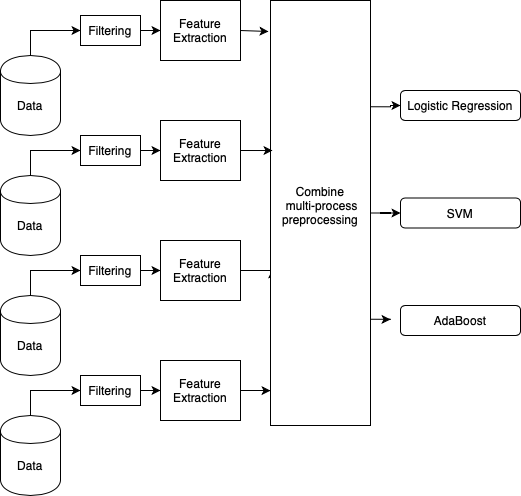
\includegraphics[width=\columnwidth]{tex/figures/model.png}
    \caption{Our Proposed Method}
    \label{fig:model}
\end{figure}

Our preliminary testing found that reading and the preprocessing stage
was very slow.
To combat this we designed a multi-processes preprocessing stage.
Here each process reads a chunk of the data and applies filtering,
feature extraction, and dimensional reduction independently.

For filtering we use a butter worth filter with various cutoffs which are dependent on the signal in which we are processing.
Band notch is used to remove power line hum and high pass filters are used to remove
baseline wander.
For feature creation we split the EEG signal into its alpha, beta, theta, and gamma bands.
From this we created the features by splitting the power from each band

For dimensional reduction we reduced the 368 dimensions using PCA
and then selecting the top 40 vectors.
Although this is a significant reduction in dimension we keep 82\% of our
original variance.

Then these processes join and are fed into 3 different classifiers;
A Logistic Regression, SVM, and KNN.
We also tried to use Naive Bayes but we were unable to get it working.
These classifiers are independent and the output of each is measured.
We also feed each output into a voting classifier.
If we had time we would have continued our multiprocessing efforts to do each
classification in parallel to further reduce run time.
